\section{Case Study Results}
\begin{figure*}
\vspace{10pt}
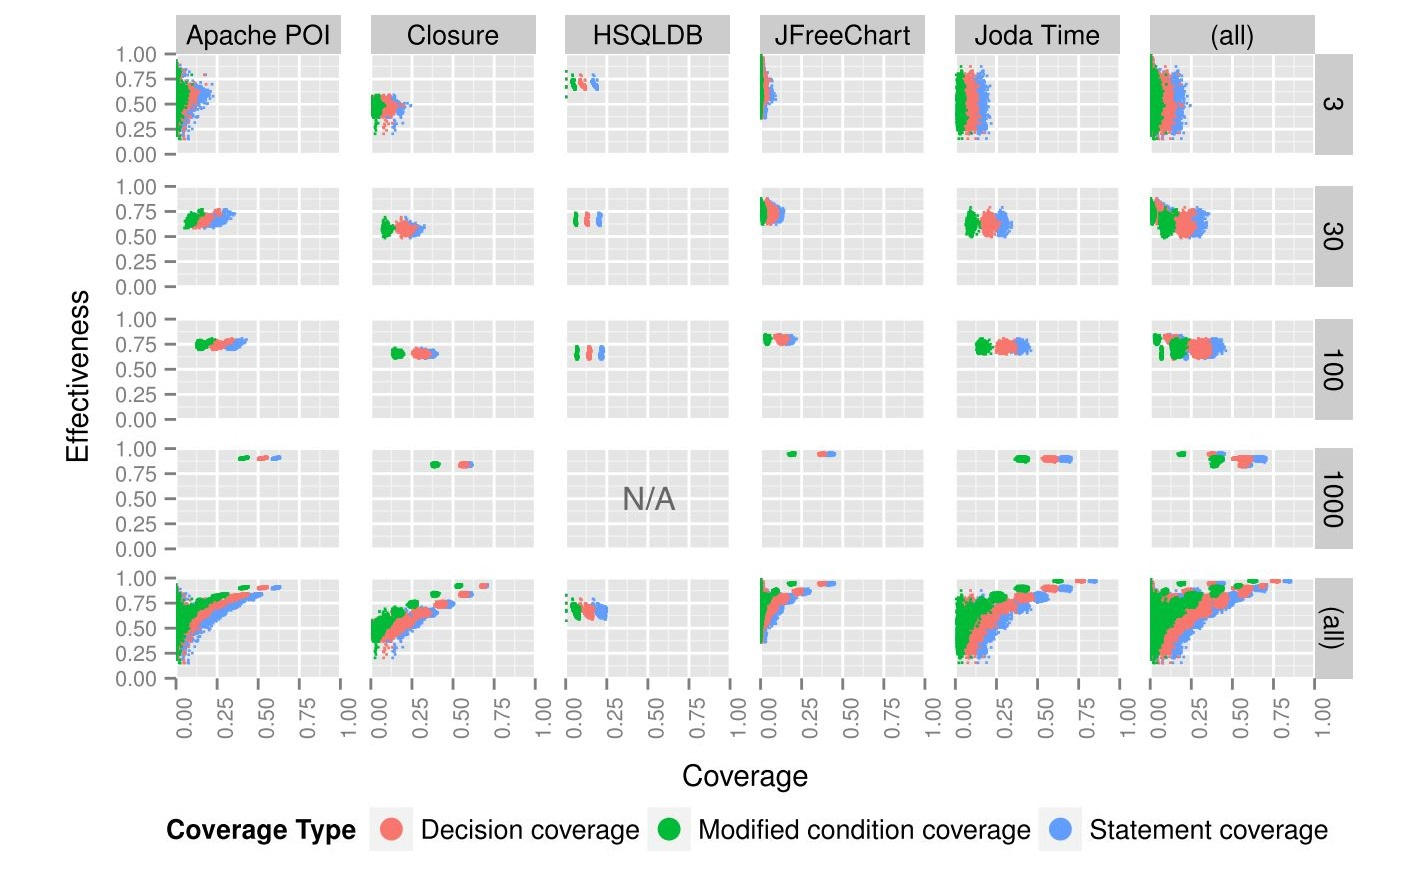
\includegraphics[width=\textwidth,height=8cm]{Figures/Coverage_result.JPG}
\caption{Normalized effectiveness scores (left axis) plotted against coverage (bottom axis) for all subjects. Rows show the results for one suite size; columns show the results for one project. N/A indicates that the project did not have enough test cases to fill in that frame.}
\label{f1}
\end{figure*}

\textbf{RQ1: Can a context-aware rank transformation provide predictive power comparable to the power of log transformation?}\\
rank transformations to the models built using log transformations. Table 1. presents the mean values of the six performance measures of both log and rank transformations, and the corresponding p-values of Wilcoxon rank sum test. The
results show the difference between the two transformations is small (i.e., less than 0.10). They concluded that rank transformation achieves comparable performance to log transformation. It is reasonable to use the proposed rank transformation method to build universal defect prediction models.\\
\textbf{RQ2: What is the performance of the universal defect
prediction model?}\\
and the AUC value. Hence, the context factors are good predictors for building a universal defect prediction model.\\
\textbf{RQ3: What is the performance of the universal defect prediction model on external projects?}\\
ble predictive power.


\begin{table}
\begin{center}
\label{tab:coverageTable}
\caption{The Kendall $\tau$ and Pearson correlations between different types of coverage for all suites from all projects.}
 \begin{tabular}{c c c} 
 \hline
 \textbf{Coverage Types} & \textbf{Kendall's }$\uptau$ & \textbf{Pearson's r}\\ [0.5ex] 
 \hline
 Statement/Decision & 0.92 & 0.99 \\ 
 
 Decision/MCC & 0.91 & 0.98 \\
 
 Statement/MCC & 0.92 & 0.97 \\
 \hline
\end{tabular}
\end{center}
\end{table}